\documentclass{standalone}
\usepackage{tikz}
\begin{document}
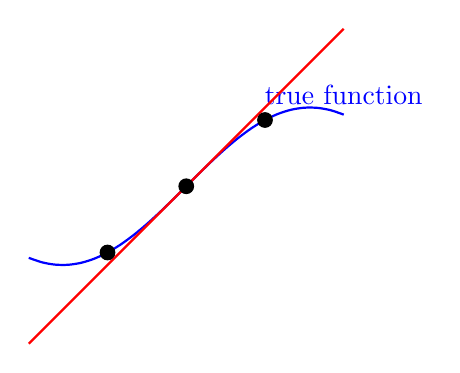
\begin{tikzpicture}[domain=-2:2,smooth,thick]
   \draw[blue] plot({\x},{sin(deg(\x))}) node[above] {true function};
   \draw[color=red] plot (\x,\x);
   \fill (1,{sin(deg(1))}) circle[radius=.1];
   \fill (0,{sin(deg(0))}) circle[radius=.1];
   \fill (-1,{sin(deg(-1))}) circle[radius=.1];
\end{tikzpicture}
%\usepackage{pgfplots}
%\usepgfplotslibrary{fillbetween}
% \begin{tikzpicture}
%     \begin{axis}[
%         width=10cm,
%         height=7.5cm,
%         xlabel={$x$},
%         ylabel={$f(x)$},
%         xmin=-2, xmax=2,
%         ymin=-2, ymax=2,
%         samples=100,
%     ]
%         % True function: f(x) = sin(x)
%         \addplot[domain=-2:2, smooth, thick, blue, dashed] {sin(deg(x))} node[above] {True function};

%       %   % Data points
%          \addplot+[only marks, red] coordinates {(-1.5, 0.9) (-1, -0.7) (0, 0) (1, 0.8)};

%       %   % Gaussian process mean
%          \addplot[domain=-2:2, smooth, thick, black] {0.2*sin(deg(2*x))} node[below] {GP mean};

%       %   % Upper confidence bound
%         \addplot[domain=-2:2, smooth, name path=upper, draw=none] {0.2*sin(deg(2*x)) + exp(-x^2)};

%       %   % Lower confidence bound
%          \addplot[domain=-2:2, smooth, name path=lower, draw=none] {0.2*sin(deg(2*x)) - exp(-x^2)};

%       % Confidence intervals
%          %\addplot[domain=-2:2, smooth, gray!50, fill opacity=0.3] fill between[of=upper and lower];


%     \end{axis}
% \end{tikzpicture}
\end{document}